\documentclass[a4paper,11pt]{article}
% --------------------------------------------------------------------------------------------------------> PACKAGES <--- %
\usepackage[frenchb]{babel}
\usepackage[utf8]{inputenc}
\usepackage{url}
\usepackage{graphicx}
\usepackage{tabularx}
\usepackage{eurosym}
\usepackage{epsfig}
\usepackage{bibtopic}
\usepackage{comment}
\usepackage{tikz}

% --------------------------------------------------------------------------------------------------------> META DATAS <--- %
\usepackage[
  colorlinks=false,
  pdfborder={0 0 0},
  pdfauthor={Emmanuel Roubin},
  pdftitle={Roubin Emmanuel | Curriculum Vitae},
  pdfsubject={Curriculum Vitae},
  pdfkeywords={Materiaux a matrice cimentaire, Milieux heterogenes, Modele morphologique, Modelisation multi-echelles, Embedded Finite Element Method},
  pdfproducer={LaTeX with hyperref package},
  pdfcreator={latex, dvips, ps2pdf}
]{hyperref}

% --------------------------------------------------------------------------------------------------------> MARGIN <--- %
\pagestyle{empty}
\usepackage{vmargin}
\setmarginsrb{1.cm}{1.5cm}{1.5cm}{1.cm}{0cm}{0cm}{0cm}{0cm}

% --------------------------------------------------------------------------------------------------------> TITLE <--- %
\newcommand{\titre}[1]{
  \begin{center}
    \rule{0.4\textwidth}{0.5pt}
    \par\vspace{0.1cm}
    \textsc{\large #1}
    \par\vspace{-0.2cm}
    \par\noindent\rule{0.4\textwidth}{0.5pt}
  \end{center}
}

% --------------------------------------------------------------------------------------------------------> BEGIN DOCUMENTS <--- %
\begin{document}
\begin{center} \par\textsc{\huge Curriculum Vit\ae} \end{center}
\begin{minipage}{0.7\linewidth}
  \begin{flushleft}
    \LARGE Emmanuel ROUBIN \normalsize  \vspace{0.1cm} \\
    \large Docteur diplômé de l'École Normale Supérieure de Cachan \normalsize\\\vspace{0.2cm}
    11 rue du commandant Debelle\\
    38000, Grenoble, France\\\vspace{0.2cm}
    %6, clos Cangina, 13\,100 Aix-en-Provence, FRANCE\\
    %Téléphone : +33 (0)6 63 04 89 29\\
    %Téléphone : +33 (0)4 56 52 86 45\\
    E-mail : \href{mailto:emmanuel.roubin@3sr-grenoble.fr}{emmanuel.roubin@3sr-grenoble.fr}\\
    Célibataire, nationalité fran\c caise, 29 ans\\
  \end{flushleft}
\end{minipage}
\hfill
\begin{minipage}{4cm}
  %\centering \fbox{\href{http://perso.crans.org/roubin}{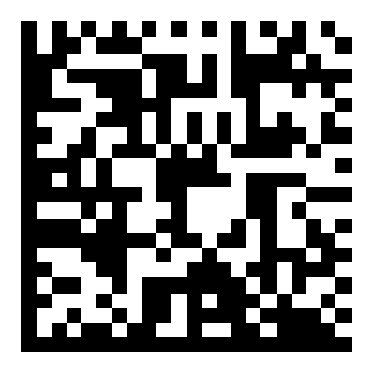
\includegraphics[width=3cm]{img/flashcode.eps}{}}}\\\vspace{0.1cm} \footnotesize\href{http://perso.crans.org/roubin}{perso.crans.org/roubin}
  \centering
  \fbox{\href{http://perso.crans.org/roubin}{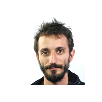
\includegraphics[width=3cm]{img/id.eps}{}}} \\ \vspace{0.1cm}
  \footnotesize\href{http://perso.crans.org/roubin}{perso.crans.org/roubin}
\end{minipage}
\vspace{0.5cm}
%\begin{center}
%  \textsc{Profil : Chercheur en Génie Civil / Numéricien / Ancien moniteur de l'ENS Cachan}
%\end{center}

% --------------------------------------------------------------------------------------------------------> PARCOURS <--- %
\titre{Parcours}
\noindent\begin{tabular}{p{0.2\textwidth}p{0.75\textwidth}m{0.1\textwidth}}
  Depuis Sept. 2015 & \textbf{Maître de conférence} de l'Université Joseph Fourier à Grenoble (UJF). Enseignant à l'IUT 1 GCCD rattaché au laboratoire 3SR.\\
  Oct. 2013 à Juin 2015 & \textbf{Post-doctorant à l'International Center for Numerical Methods in Engineering (CIMNE)}, UPC Barcelone (Espagne), chez le Professeur X. Oliver. Travail au sein de l'équipe du projet ERC \emph{Advanced tools for computational design of engineering materials}  \hfill \raisebox{-0.2cm}{\epsfig{figure=img/flag_catalan, height=0.6cm}} \\ 
  Octobre 2013  & \textbf{Docteur} de l'ENS~Cachan. Sujet : \textit{Modélisation EF et morphologique de milieux hétérogènes à l'échelle mésoscopique : applications aux matériaux à matrice cimentaire}. Doctorat effectué sous la direction \href{http://lml.univ-lille1.fr/lml/?page=15&manID=1839}{J.-B. Colliat (LML, Lille)} au LMT-Cachan. Thèse soutenue à l'ENS Cachan le 10/10/2013 devant le jury composé de N. Burlion (président), D. Kondo (examinateur), J.-M. Torrenti (examinateur), X. Oliver, N. Benkemoun et J.-B. Colliat. \\ 
  Mai - Juin 2012  &  \textbf{Séjour à l’Institut für Wissenschaftliches Rechnen}, TU Braunschweig (Allemagne), chez le Professeur H.G. Matthies. \hfill \raisebox{-0.2cm}{\epsfig{figure=img/flag_german, height=0.6cm}} \\ 
  Sept. 2011 à 2013 & \textbf{Doctorant} chargé d'une \textbf{mission d'enseignement} à l'ENS~Cachan (128h)\\ 
  Sept. 2010 à 2011 & \textbf{Doctorant} et \textbf{vacataire} à l'ENS~Cachan (56h)\\ 
  Juin 2010      & \textbf{Diplôme de Master Recherche Génie Civil} de l'ENS~Cachan : Structures, Ouvrages et Matériaux dans leur environnement\\
                 & \textbf{Diplôme de l'ENS~Cachan}\\ 
  Mars - Juin 2010 & \textbf{Stage de recherche} (M2) au LMT-Cachan. Sujet : \textit{Modélisation morphologique des matériaux hétérogènes} sous la direction de J.-B. Colliat.\\
  Mai - Juillet 2009 & \textbf{Stage de recherche} (M1) à l'Université de Canterbury (Nouvelle-Zélande). Sujet : \textit{Evaluation of Screws Used in Laminated Veneer Lumber Rocking Connections} sous la direction de A.H. Buchanan. \hfill \raisebox{-0.2cm}{\epsfig{figure=img/flag_nz, height=0.6cm}} \\
  Septembre 2006 & Élève \textbf{professeur stagiaire} à l'ENS~Cachan (normalien)\par Physique appliquée puis Mécanique, Génie Civil  \\ 
  De 2004 à 2006 &  \textbf{Classes préparatoires} PT/PTSI (Lycées Vauvenarges, Aix-en-Provence)
\end{tabular}
\vfill

% --------------------------------------------------------------------------------------------------------> ENSEIGNEMENT <--- %
\titre{Activités pédagogiques}
\begin{itemize}
\item[\textbf{Enseignements}]:
  \begin{itemize}
  \item Depuis 2015, \textbf{MCF} en l'IUT GCCD principalement en géotechnique.
  \item 2010 - 2013, \textbf{vacataire} puis chargé d'une \textbf{mission d'enseignement} à l'ENS Cachan et à l'UPMC (Jussieu Paris VI) pour un total de \textbf{184h eq. TD}. (Probabilité et incertitudes, Mécanique des Milieux Continus, Méthodes numériques, Mécanique probabiliste\dots
  \end{itemize}
  \item[\textbf{Projet pédagogique:}] Création de TD en L3, M1 et M2 suivant un plan pédagogique uniforme autour de la thématique \og\emph{découverte de la modélisation et de l’analyse des phénomènes aléatoires en mécanique}\fg.\\
  \item[\textbf{Actions collectives:}] Encadrement d'ateliers de vulgarisation scientifique lors des journées portes ouvertes de l'ENS Cachan au département de Génie-Civil (2011).\\
\end{itemize}
\vfill

% --------------------------------------------------------------------------------------------------------> RECHERCHE <--- %
\titre{Activités de recherche}
% ---> CNRS <---
\begin{comment}
  \begin{itemize}
    \item[\textbf{Thématiques}] :
    \item Modélisation analytique et numérique du caractère aléatoire de la \textbf{morphologie des milieux hétérogènes}
    \item Modélisation numérique du \textbf{comportement quasi-fragile des matériaux à matrice cimentaire}
    \item Analyse multi-échelles et \textbf{multi-physiques} des matériaux hétérogènes
    \item Procédures de \textbf{réduction de modèles} à hautes performances appliquées à des champs discontinus
      %\item[Mots clefs :]
      %\item Matériaux à matrice cimentaire, Milieux hétérogènes, Modèle morphologique, Modélisation multi-échelles, Fissuration, \textit{Embedded Finite Element Method}\\
    \item[\textbf{Projets en cours}] :
    \item I+D+I : Participation à l'élaboration et à la demande de financement du projet national espagnol (I+D+I) \textit{``Computational design of engineering materials subjected to dynamic actions''} porté par O. Llobera-Valls en tant que chercheur associé.
    \item ERC : Participation au projet Européen ERC \textit{``Advanced tools for computational design of engineering materials''} porté par X. Oliver en tant que post-doctorant.
    \item[\textbf{Encadrements}] :
    \item 1 stage de M2 : \textit{Modèle morphologique d'hydratation de matrices cimentaires} M. Bogdan, (2011, 50\%)
    \item 3 projets de M2 : C. Mathey (2010, 100\%), M. Bogdan (2011, 30\%), P.-J. Pouit (2011, 100\%) 
    \item[\textbf{Principales contributions}] :
      \begin{btSect}[bib/chrono]{bib/Published_short}
        \btPrintAll
      \end{btSect}
    \item[\textbf{Conférences internationnales}] : 
    \item Présentation orale: WCCM (Espagne, 2014), WCCM (Brésil, 2012), COMPLAS (Espagne, 2011)
    \item Co-auteur: EURO-C (X. Oliver, Autriche, 2014), Micro-durability (M. Bogdan, Hollande, 2012)
  \end{itemize}
\end{comment}
% ---> MCF <---
\begin{itemize}
  \item[\textbf{Thématiques}] : Modélisation numérique du comportement des bétons
    \begin{itemize}
    \item Modélisation du caractère aléatoire de la \textbf{morphologie} (inclusions, porosité)
    \item Analyse \textbf{multi-échelles} et \textbf{multi-physiques}
    \item Modélisation de la \textbf{fissuration} et procédures de \textbf{réduction de modèles}
    \item Percolation
    \end{itemize}
  \item[\textbf{Projets}] :
  \item 2015 - : Participation à l'ANR MOSAIC \textit{``MesOscopic Scale durAbility Investigations for Concrete''} portée par J.-B Colliat.
  \item 2014 - : Participation au projet national espagnol (I+D+I) \textit{``Computational design of engineering materials subjected to dynamic actions''} porté par O. Llobera-Valls en tant que chercheur associé.
  \item 2013 - : Participation au projet Européen ERC \textit{``Advanced tools for computational design of engineering materials''} porté par X. Oliver en tant que post-doctorant.
  \item[\textbf{Encadrements}] :
  \item Thèse Paul Hauseux : \textit{``Modélisation des la fissuration et propagation des incertitudes au travers de Méthodes Éléments Finis: Applications à des probèmes d'excavation.''}
  \item Thèse Alexis Vallade : \textit{``Modélisation multi-échelle du gaz de schiste. Influence de la microstructure sur les propriétés macroscopiques et le procesus de fracturation.''}
  \item 1 stage de M2 et 3 projets de M2 : C. Mathey (2010), M. Bogdan (2011), P.-J. Pouit (2011) 
  \item[\textbf{Principales contributions}] :
    \begin{btSect}[bib/chrono]{bib/Published_short}
      \btPrintAll
    \end{btSect}
  \item[\textbf{Conférences internationnales}] : 
  \item Présentation orale: WCCM (Espagne, 2014), WCCM (Brésil, 2012), COMPLAS (Espagne, 2011)
  \item Co-auteur: EURO-C (X. Oliver, Autriche, 2014), Micro-durability (M. Bogdan, Hollande, 2012)
\end{itemize}
\vfill

% --------------------------------------------------------------------------------------------------------> COMPETENCES <--- %
\titre{Compétences}
\begin{tabular}{p{0.18\textwidth}b{0.01\textwidth}p{0.8\textwidth}}
  \textbf{Langues} & : & \textbf{Fran\c cais} (natif), \textbf{Anglais} (courant), Espagnol et Italien\\
  \textbf{Programmation} & : & $C$, $C++$, Fortran77, Python, Bash, Web (PHP, MySql)\\
  \textbf{Logiciels} & : & Feap (code EF), Matlab, cran-R (statistiques)\\
                     &   & Travail sous environnement Unix/Linux\\
  \textbf{Edition} & : & \LaTeX, Pack Office, Web (html5, css3, Jquery)
\end{tabular}
\vfill

% --------------------------------------------------------------------------------------------------------> INVESTISSEMENTS <--- %
\titre{Activités diverses}

\begin{tabular}{lcp{0.8\linewidth}}
  2014      & : & Développement du site internet d'apprentissage du fran\c{c}ais \href{http://e2lf.fr}{E2LF}\\
  2010      & : & Développement du site internet de \href{http://www.ecoba.ens-cachan.fr/index.php?part=acces}{l'ANR blanc ECOBA}\\
  2008      & : & Assistant régisseur lunière à l'Européen (Paris)\\
  2007-2008 & : & Président de deux associations culturelles (BdA/SdA Cachan)\\ 
  2007      & : & Elaboration et réalisation d'un projet éducatif en Inde (Hoé-Inde)\\
\end{tabular}

\vspace{0.5cm}
\begin{tabular}{lcp{0.8\linewidth}}
  \textbf{Sport} & : & Escalade et sports de haute-montagne\\
  \textbf{Musique} & : & Médaille d'or du conservatoire  Darius Milhaud en violoncelle (Aix-en-Provence 2004)\\
                   &  & saxophone\\
  \textbf{Autre} & : & Speedcuber, Webmaster, Régie lumière, photographie
\end{tabular}

\vfill
\empty
	
\end{document}
